%=========================================================================
% (c) Radim Loskot, 2014

\chapter{Obsah přiloženého DVD}
\label{Annex.dvdContent}


Elektronický nosič obsahuje pracovní adresář pro vývojové prostředí Eclipse Kepler. Implementované rozšíření se nachází ve složce projektu \textbf{ScriptBox/}. Ostatní projekty umístěné v adresáři jsou zapotřebí ke správné kompilaci knihovny rozšíření. Manuál ke kompilaci knihovny lze nalézt buď v souboru \textbf{README}, v příloze \ref{Annex.manual} nebo na stránkách repozitáře projektu\footnote{\url{https://github.com/ITman1/ScriptBox}}.

\medskip

\noindent Na elektronický nosič byly přiloženy následující součásti diplomové práce: 
\bigskip

\begin{itemize}
  \item \textbf{CSSBox/} -- (X)HTML renderovací knihovna;
  \item \textbf{CSSParser/} -- parser kaskádových stylů;
  \item \textbf{Doc/} -- technická zpráva;
    \begin{itemize}
      \item \textbf{zprava.pdf} -- technická zpráva ve formátu PDF;
    \end{itemize}
  \item \textbf{ScriptBox/} -- rozšíření skriptování v (X)HTML dokumentech;
    \begin{itemize}
      \item \textbf{demo/} -- zdrojové kódy ukázkových HTML stránek;
      \item \textbf{doc/} -- programová dokumentace knihovny v HTML formátu;
      \item \textbf{src/} -- zdrojové kódy knihovny a testů rozšíření;
      \item \textbf{target/} -- výstupní složka pro sestavenou knihovnu;
      \item \textbf{README} -- instalační manuál;
    \end{itemize}
  \item \textbf{SwingBox/} -- prohlížeč webových stránek využívající CSSBox.
\end{itemize}

\chapter{Předzpracování skriptu}
\label{Annex.ScriptPreprocessing}

\begin{figure}[H]
  \begin{center}
    \scalebox{0.63}{
      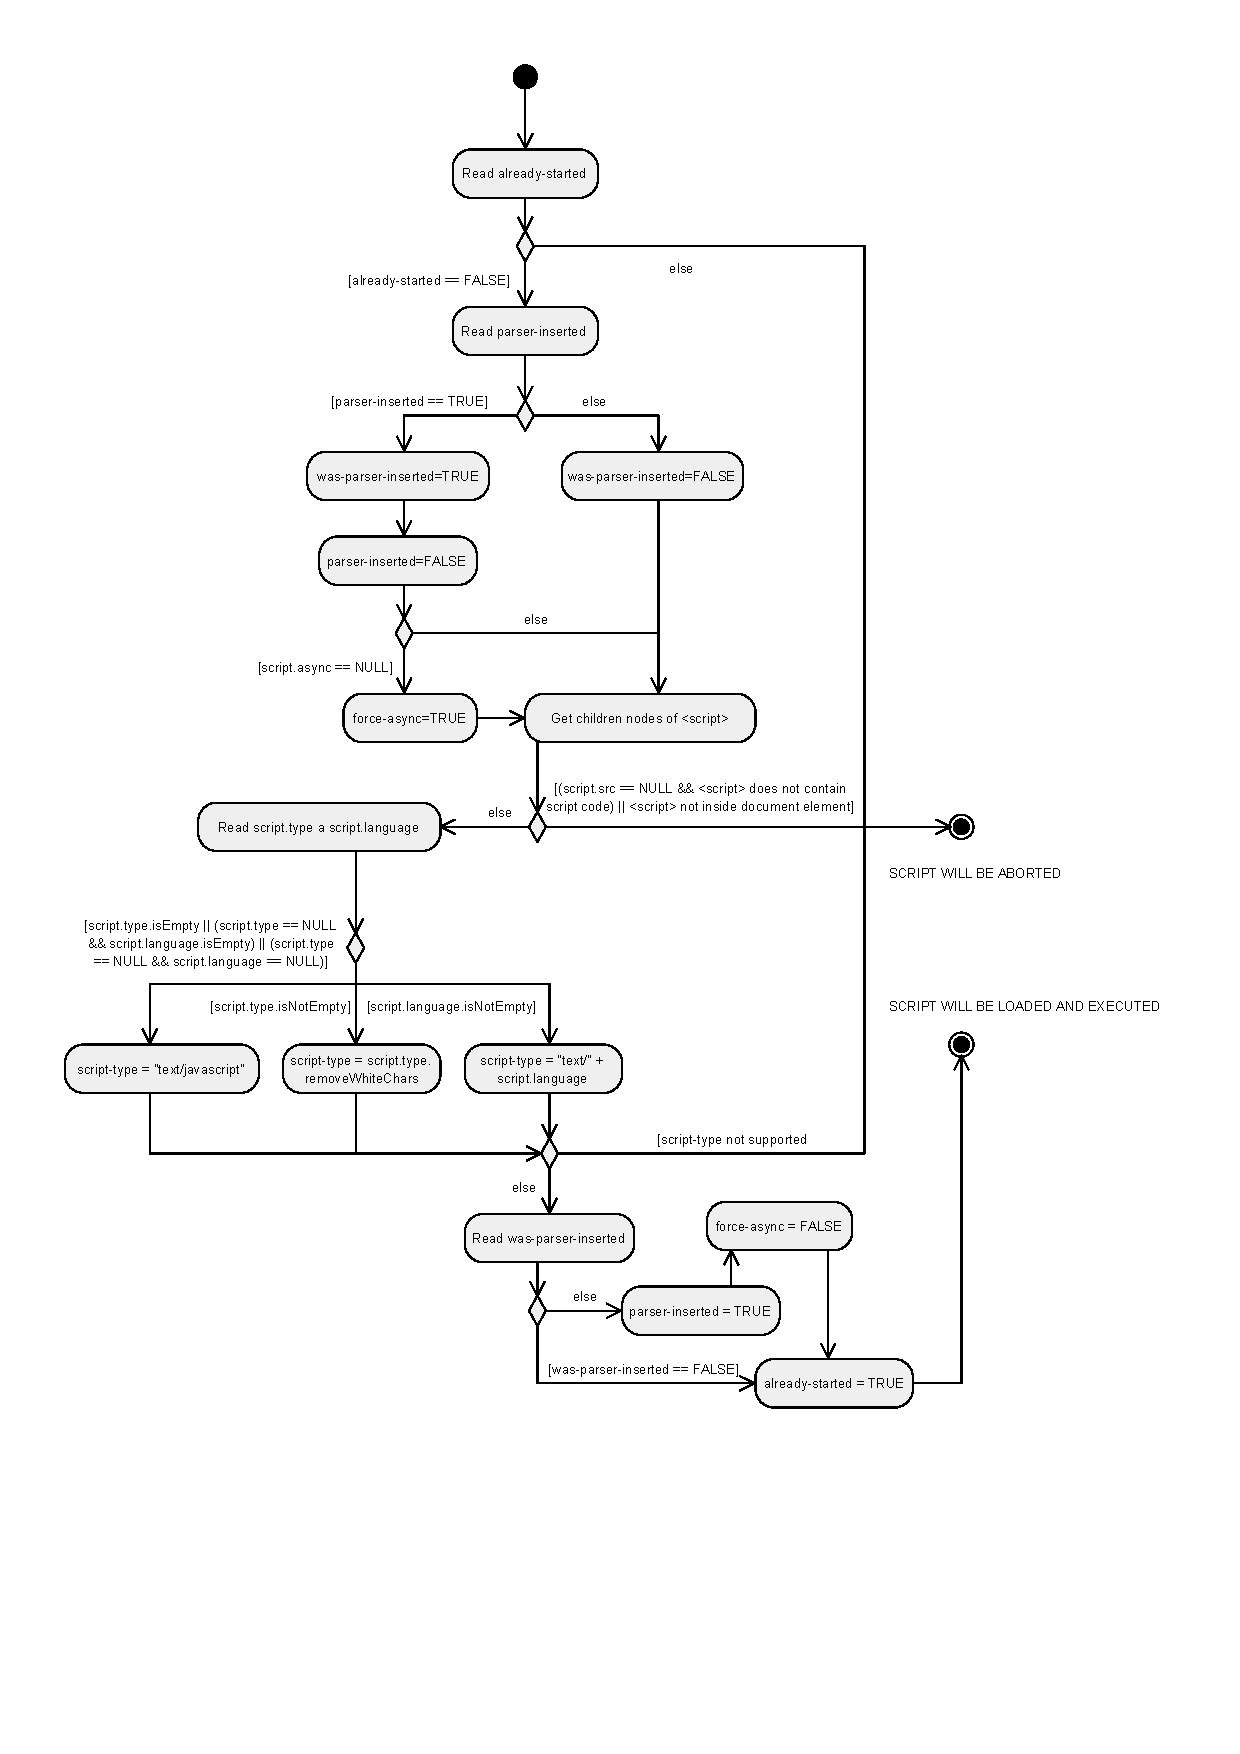
\includegraphics{fig/script-preparation-steps.pdf}
    }
    \caption{Diagram aktivit znázorňující kroky přípravy skriptu před jeho vykonáním}
    \label{Figure.ScriptPreparationSteps}
  \end{center}
\end{figure}

\chapter{Manuál}
\label{Annex.manual}

Knihovnu rozšíření lze přeložit více způsoby. Nejběžnější dva způsoby uvedeme v této příloze.

Pokud máme k dispozici přiložené DVD k této práci, lze překlad provést ve vývojovém prostředí Eclipse Kepler s integrovaným nástrojem Maven\footnote{\url{http://maven.apache.org/}}. K překladu knihovny je mít projekty pracovního adresáře (CSSBox, CSSParser a SwingBox) zkompilováné a nainstalované nástrojem Maven (Run -> Run As -> Maven install). Nainstalováním se přidají knihovny těchto projektů do lokálního repozitáře nástroje Maven. Jakmile jsou knihovny nainstalovány, bude možno v Eclipse provést překlad implementovaného rozšíření -- projektu ScriptBox.

Nevlastníme-li přiložené DVD a předpokládejme i vývojové prostředí Eclipse, je zapotřebí požadované projekty stáhnout a nainstalovat manuálně. Pro manuální překlad knihovny platí následující předpoklady:

\begin{itemize}
  \item Nainstalované JDK 1.6 nebo novější, kde JDK 1.8 je doporučeno,
  \item Nainstalovaný sestavovací systém Maven,
  \item Vytvořená systémová proměnná \texttt{JAVA\_HOME} ukazující na lokaci JDK,
  \item Přidaná cesta v systémové proměnné \texttt{PATH} k binárním souborům JDK,
  \item Přidaná cesta v systémové proměnné \texttt{PATH} k binárním souborům nástroje Maven,
  \item Naklonován repozitář projektu CSSBox \footnote{\url{https://github.com/radkovo/CSSBox}},
  \item Naklonován repozitář projektu CSSParser\footnote{\url{https://github.com/radkovo/jStyleParser}},
  \item Naklonován repozitář projektu SwingBox\footnote{\url{https://github.com/radkovo/SwingBox}},
  \item Mít sestavené a nainstalované knihovny projektů CSSBox, CSSParser a SwingBox v~lokálním repozitáři nástroje Maven.
\end{itemize}

Jakmile jsou všechny předpoklady splněny, překlad provedeme příkazem \texttt{mvn package}. Během překladu se nástrojem Maven stáhnou také další zbývající závislosti. 

\chapter{Metriky kódu knihovny}
\label{Annex.metrics}

Pro získání některých měr bylo využito nástroje Metrics\footnote{\url{http://metrics.sourceforge.net/}}.

\begin{itemize}
  \item \textbf{velikost sestavené knihovny} -- XY kB;
  \item \textbf{počet řádků} -- $37400$;
  \item \textbf{počet řádků (bez komentářů a bílých znaků)} -- $19249$;
  \item \textbf{počet řádků (uvnitř těl metod)} -- $8981$;
  \item \textbf{počet balíků} -- $45$;
  \item \textbf{počet tříd} -- $266$;
  \item \textbf{počet atributů} -- $620$;
  \item \textbf{počet metod} -- $2200$;
  \item \textbf{počet odvozených tříd} -- $133$;
  \item \textbf{počet přepsaných metod} -- $337$;
  \item \textbf{hloubka stromu dědičnosti (arit. průměr; směr. odchylka)} -- $(2,21; 1,27)$;
  \item \textbf{eferentní propojení balíčků} -- $(1,57;2,80)$;
  \item \textbf{aferentní propojení balíčků} -- $(9,53;10,73)$;
  \item \textbf{nedostatečná soudružnost v metodách} -- $(0,21;0,32)$;
  \item \textbf{McCabe cyklomatická složitost} -- $(1,57;2,00)$;
\end{itemize}

\chapter{Aplikace jednoduchého prohlížeče}
\label{Annex.SimpleBrowser}

\begin{figure}[H]
  \begin{center}
    \scalebox{0.55}{
      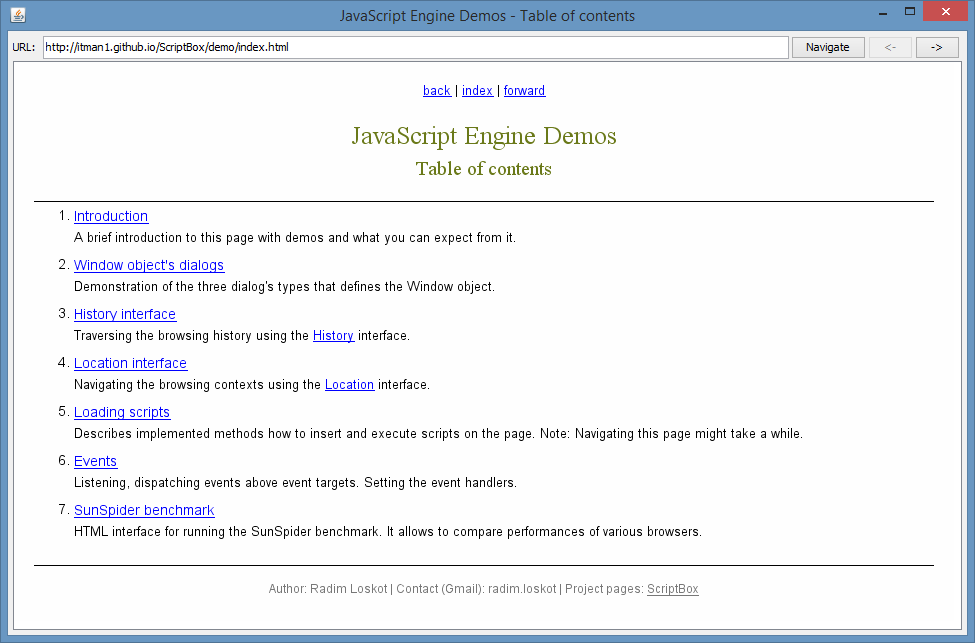
\includegraphics{fig/browser.png}
    }
    \caption{Uživatelské rozhraní jednoduchého prohlížeče}
    \label{Figure.SimpleBrowserScreenshot}
  \end{center}
\end{figure}

\chapter{Aplikace testeru JavaScriptu}
\label{Annex.JavaScriptTester}

\begin{figure}[H]
  \begin{center}
    \scalebox{0.45}{
      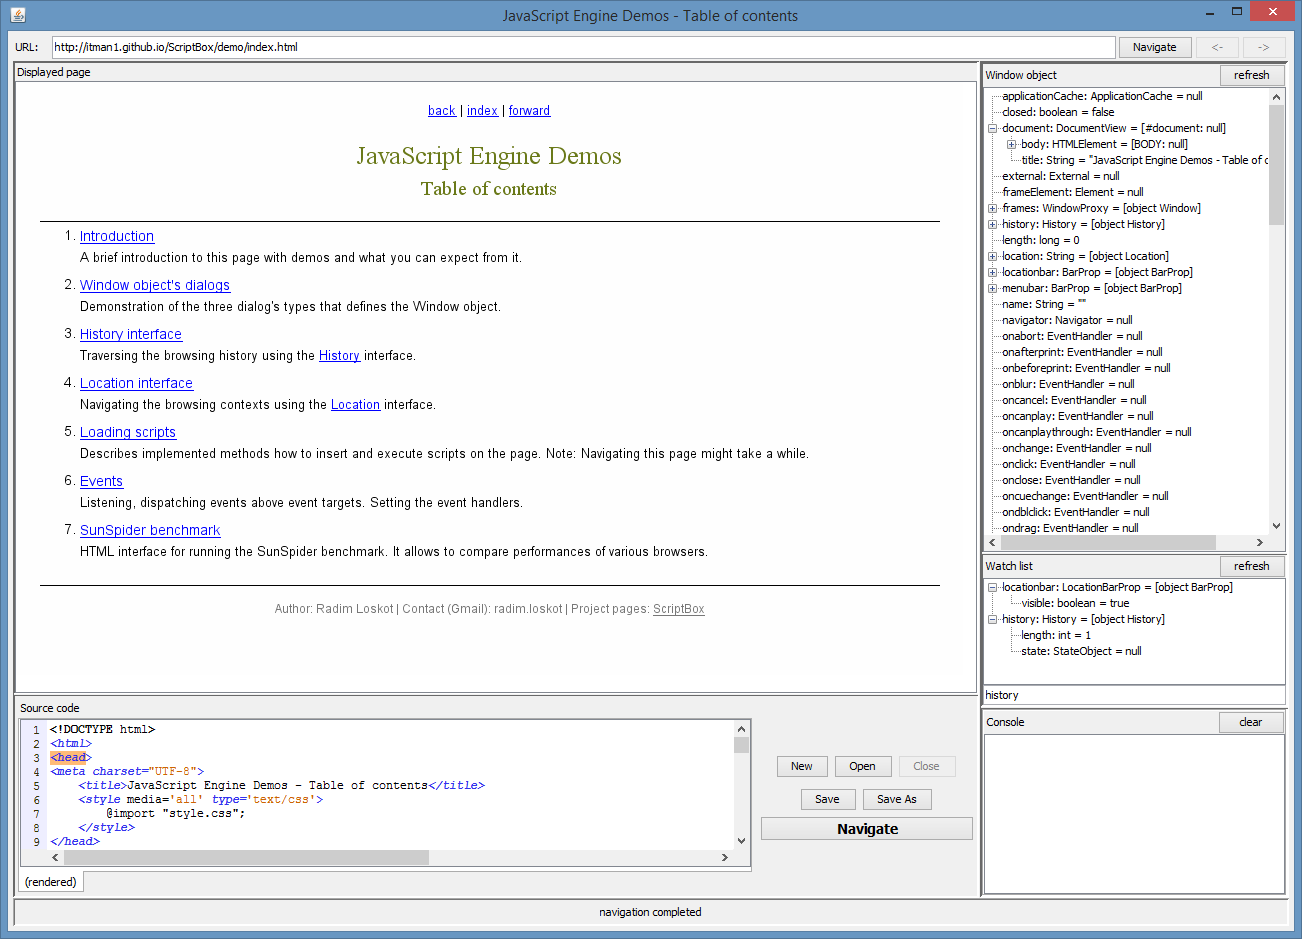
\includegraphics{fig/tester.png}
    }
    \caption{Uživatelské rozhraní aplikace JavaScriptového testeru}
    \label{Figure.JavaScriptTester}
  \end{center}
\end{figure}

\chapter{Popis balíků knihovny}
\label{Annex.packageDescription}

Následující seznam obsahuje popis nejdůležitějších balíků projektů. Z cest balíků byla vynechána 
cesta k hlavního balíku projektu \texttt{org/fit/cssbox/scriptbox}.

\bigskip

\noindent Výčet nejdůležitějších balíků knihovny:

\begin{itemize}
  \item \textbf{browser/} -- jádro uživatelského agenta (uživatelský agent, procházecí jednotka a jednotlivé podporované procházecí kontexty);
  \item \textbf{demo/} -- ukázkové aplikace knihovny;
     \begin{itemize}
       \item[] \textbf{browser/} -- aplikace jednoduchého prohlížeče;
       \item[] \textbf{tester/} -- aplikace testeru JavaScriptu;
     \end{itemize}
  \item \textbf{dom/} -- třídy objektového modelu DOM (uzly, výjimky, události);
     \begin{itemize}
       \item[] \textbf{events/} -- třídy reprezentující události DOM;
         \begin{itemize}
           \item[] \textbf{adapters/} -- adaptéry událostí Xerces na události viditelné ve skriptech;
           \item[] \textbf{script/} -- třídy událostí viditelných ve skriptech;
         \end{itemize}
       \item[] \textbf{interfaces/} -- rozhraní uzlů dokumentu;
     \end{itemize}
  \item \textbf{events/} -- událostní smyčka jádra, plánovače úloh a abstraktní třída úlohy;
  \item \textbf{exceptions/} -- výjimky jádra uživatelského agenta;
  \item \textbf{history/} -- procházení historie (historie sezení, záznam historie, společná historie sezení a rozhraní \texttt{History});
  \item \textbf{misc/} -- pomocné třídy knihovny;
  \item \textbf{navigation/} -- navigace mezi dokumenty (navigační kontroler, navigační požadavky a rozhraní \texttt{Location});
  \item \textbf{parser/} -- parser dokumentu a úloha zajišťující kompletizaci parsování;
  \newpage
  \item \textbf{reource/} -- stahování a zpracovávání obsahu zdroje;
     \begin{itemize}
       \item[] \textbf{content/} -- registr ovladačů pro zpracování obsahu;
         \begin{itemize}
           \item[] \textbf{handlers/} -- ovladače pro zpracovávání obsahu;
         \end{itemize}
       \item[] \textbf{fetch/} -- registr ovladačů pro stažení zdroje;
         \begin{itemize}
           \item[] \textbf{handlers/} -- ovladače pro stažení zdroje;
         \end{itemize}
     \end{itemize}
  \item \textbf{script/} -- skriptovací architektura;
     \begin{itemize}
       \item[] \textbf{adapter/} -- registr adaptérů;
       \item[] \textbf{annotation/} -- skriptovací anotace pro export objektů;
       \item[] \textbf{exceptions/} -- výjimky způsobené jádrem pro skriptování;
       \item[] \textbf{injectors/} -- injektory společné pro více skriptovacích enginů;
       \item[] \textbf{javascript/} -- implementace skriptovacího enginu JavaScriptu;
         \begin{itemize}
           \item[] \textbf{injectors/} -- injektory skriptovacího enginu JavaScriptu;
           \item[] \textbf{java/} -- implementátor globálního scopu JavaScriptu a obaly nativních objektů, atributů a metod;
           \item[] \textbf{wrap/} -- obalovací továrny podporované enginem;
         \end{itemize}
       \item[] \textbf{reflect/} -- obaly členů tříd Javy -- reflexe;
     \end{itemize}
  \item \textbf{security/} -- třídy pro bezpečnostní kontroly;
     \begin{itemize}
       \item[] \textbf{origins/} -- pomocné třídy Origin pro určení původu obsahu zdroje;
     \end{itemize}
  \item \textbf{ui/} -- rozšíření uživatelského agenta o grafické rozhraní;
  \item \textbf{url/} -- třídy pro práci s URL;
  \item \textbf{window/} -- implementace globální objektu \texttt{Window} a jeho proxy \texttt{WindowProxy}.
\end{itemize} 


%\chapter{Konfigrační soubor}
%\chapter{RelaxNG Schéma konfiguračního soboru}
%\chapter{Plakat}

